% Chapter Template

\chapter{Estat de l'art} % Main chapter title

\label{Chapter2} % Change X to a consecutive number; for referencing this chapter elsewhere, use \ref{ChapterX}

Per conèixer millor el potencial d'aquest mercat i saber les alternatives per a una major profunditat en el coneixement del sector, s'ha de realitzar un estudi del mercat existent per a comprovar la presència d'aplicacions que són similars, sigui per objectiu o per mercat, a \textit{Wisebite}. A continuació apareixen algunes de les aplicacions que s'han pogut trobar.
\\\\
El fet d'analitzar cadascuna d'elles et permet veure quines funcionalitats pots oferir al client perquè directament no existeix cap eina que les faciliti o bé per millorar les existents. S'ha volgut destacar sis plataformes similars a \textit{Wisebite}, algunes en millors aspectes que altres. Al acabar de valorar cadascuna d'elles, es realitzarà un estudi ja més globalitzat que permeti veure quines avantatges ofereix \textit{Wisebite} al mercat actual.

%----------------------------------------------------------------------------------------
%	SECTION 1
%----------------------------------------------------------------------------------------

\section{Waiterio}

Aplicació\cite{waiterio} orientada especialment a substituir el \textit{TPV} d'un bar o restaurant. Disposa de funcionalitats com creació de menús i comandes, convidar companys de feina amb rols associats, visualització en mòbil i tauleta, reports periòdics i generació de factures totals o fraccionades.
\\\\
L'aplicació disposa d'entre unes 50.000 i 100.000 descàrregues al \textit{Play Store}. En general, conté moltes funcionalitats i té una interfície d'usuari ben cuidada que permet l'ús de l'aplicació de forma més còmode i confortable.
\\
\begin{figure}[H]
\centering
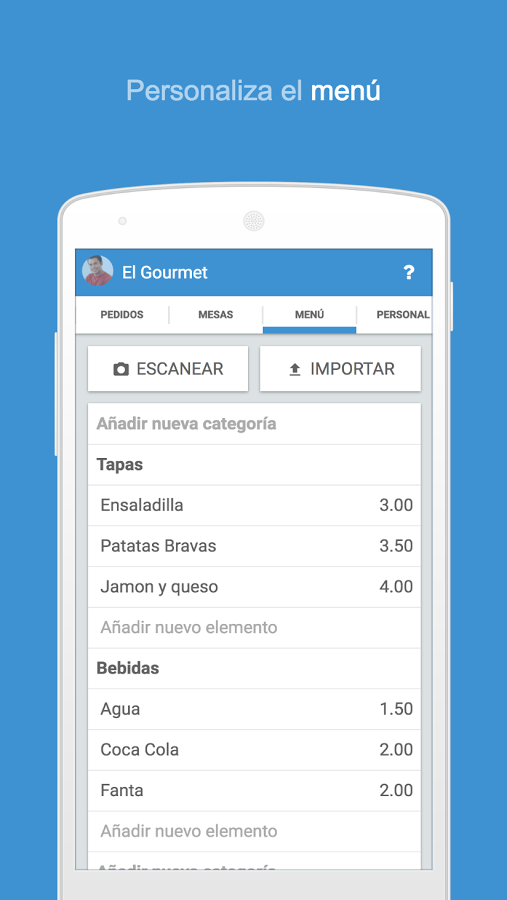
\includegraphics[scale=0.15]{Figures/waitero-1.png}
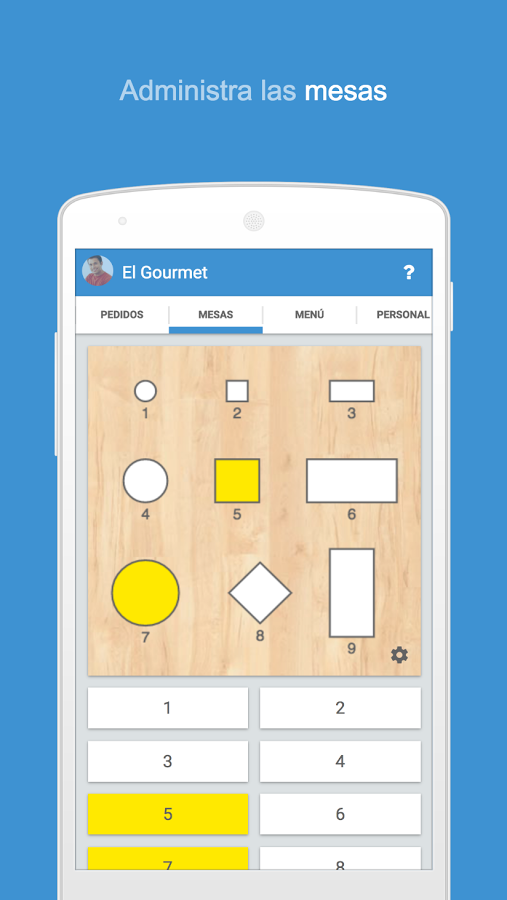
\includegraphics[scale=0.15]{Figures/waitero-2.png}
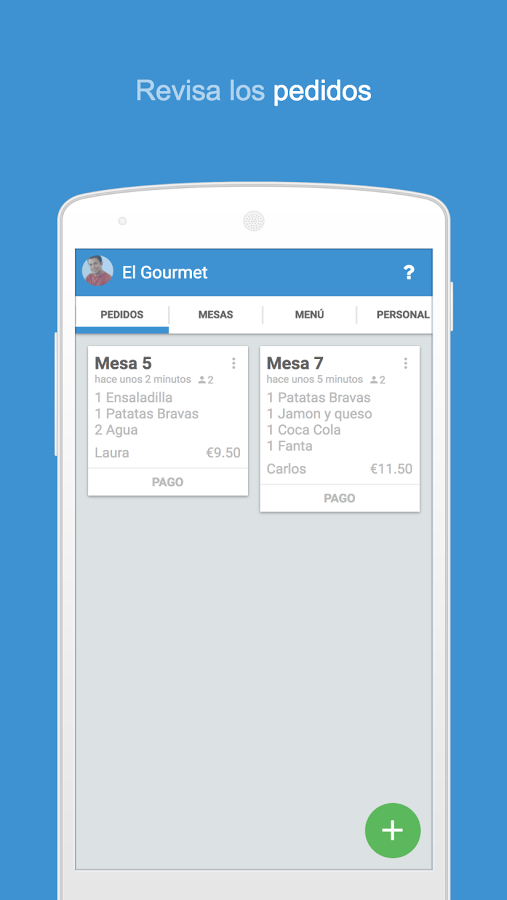
\includegraphics[scale=0.15]{Figures/waitero-3.png}
\caption{Captures de pantalla de Waitero}
\end{figure}



%----------------------------------------------------------------------------------------
%	SECTION 2
%----------------------------------------------------------------------------------------

\section{Prime Tray}

Aplicació\cite{primetray} orientada a les comandes del client a l'establiment. L'usuari té la capacitat de seleccionar un restaurant de la llista i fer la comanda en línia i anar-ho a buscar un cop és notificat.

%----------------------------------------------------------------------------------------
%	SECTION 3
%----------------------------------------------------------------------------------------

\section{OrderSev}

Aplicació\cite{ordersev} orientada especialment a substituir el TPV d'un bar o restaurant. Disposa de funcionalitats com creació de menús i comandes, generació de factures i vistes tant des de cuina com del cambrer.

%----------------------------------------------------------------------------------------
%	SECTION 4
%----------------------------------------------------------------------------------------

\section{TabletWaiter}

Aplicació\cite{tabletwaiter} orientada a ser un estil de carta per a l'establiment. Cada taula d'un restaurant hauria d'haver-hi un dispositiu amb aquesta aplicació activa a on es pugui consultar els plats i seleccionar-los, així es rebria a cuina i ja podrien començar a preparar la comanda. També permet cridar al cambrer via aplicació i demanar el compte.

%----------------------------------------------------------------------------------------
%	SECTION 5
%----------------------------------------------------------------------------------------

\section{Cloud Waiter}

Aplicació\cite{cloudwaiter} orientada a les comandes del client a l'establiment. L'usuari té la capacitat d'escanejar un codi QR amb el qual podrà accedir a l'aplicació i realitzar la comanda.

%----------------------------------------------------------------------------------------
%	SECTION 6
%----------------------------------------------------------------------------------------

\section{FastOrder}

Aplicació\cite{fastorder} orientada a les comandes del client a l'establiment. L'usuari té la capacitat d'escanejar un codi QR amb el qual podrà accedir a l'aplicació i realitzar la comanda i tot el que sigui necessari. Destacar la molt bona interfície d'usuari, que permet gaudir d'una millor experiència com a usuari.

%----------------------------------------------------------------------------------------
%	SECTION 7
%----------------------------------------------------------------------------------------

\section{Conclusions}

Encara que hi ha moltes aplicacions relacionades amb aquest àmbit (si bé, amb objectius i funcionalitats molt diverses, en alguns casos molt dispars al projecte), s'ha fet una selecció prou representativa però tot i així reduïda, amb l'objectiu de realitzar una correcta anàlisi que permeti treure conclusions de forma còmoda i eficaç.
\\\\
Un cop realitzada aquesta selecció de potencials competidors de l'aplicació, i comprès (a grans trets) les seves funcionalitats i objectius, procedim a un estudi detallat comparant-ho amb la visió d'aquest projecte.
\\\\
El que s'ha pogut veure estudiant el mercat és que hi ha dos grans grups d'aplicacions. Per una banda, tenim els sistemes que només se centren en la gestió interna de l'establiment i poder realitzar comandes més fàcil i eficientment. Per altra banda, tenim les plataformes que permeten al client, que acudeix a l'establiment, viure una millor experiència i estar còmode en la seva estança. Aleshores, partint d'aquesta premissa, \textit{Wisebite} vol innovar en el mercat oferint un nou sistema que fusioni els dos grups, així creant un fort vincle entre ambdues parts: empleat i client.